We have seen that the complete-within-a-bound approach of DPOR is not
suitable for some programs.  Programs with large state-spaces, or with
sources of nondeterminism other than the scheduler, pose a problem.
One way to address this is to sacrifice completeness, and instead
explore the space of schedules \emph{randomly}.  We may not find all
bugs.  However we still want to find \emph{most of them}.  Benchmarks
show that some scheduling algorithms tend to be better at this than
others; not all algorithms are created equal.  In this chapter we
discuss two different randomised scheduling
algorithms~\sref{algorithms-usual} and then propose a new one based on
a \emph{weighted} random selection of threads~\sref{algorithms-swarm}.
We show that our proposed algorithm performs favourably in a
comparison of standard benchmark programs~\sref{algorithms-bench}, and
evaluate the approach~\sref{algorithms-eval}.

\section{Concurrency Testing with Randomised Scheduling}
\label{sec:algorithms-usual}

Concurrency testing using randomised scheduling works by repeatedly
executing a concurrent program, exploring a particular schedule on
each execution.  Unlike systematic testing, these algorithms are
incomplete in general, and little effort is made to avoid repetition
of schedules.  In this section we present two approaches to randomised
scheduling.

\paragraph{Controlled random scheduling}
A controlled random scheduler uses a pseudorandom number generator to
choose threads to execute.  At each scheduling point, a runnable
thread is selected at random.  This thread is then executed until the
next scheduling point.  Like any controlled scheduling technique, the
executed schedule can be recorded and replayed.  Additionally, a
controlled random scheduler can be used on programs that exhibit
nondeterminism beyond scheduler nondeterminism, although in this case
schedule replay will be unreliable \parencite{thomson2016}.

\paragraph{Probabilistic concurrency testing}
The PCT algorithm \parencite{burckhardt2010} is a randomised algorithm
with a probabilistic guarantee of finding bugs.  Key to its design is
a notion of the \emph{depth} of a bug: the minimum number of
scheduling constraints required to exhibit it.  The intuition behind
PCT is that most concurrency bugs can be exhibited with just a few
scheduling decisions being made in the correct places, or the
incorrect places depending on your point of view.  If PCT makes those
decisions correctly, it finds the bug regardless of what any other
scheduling decisions were.

On each execution, PCT focuses on finding bugs of a particular depth
$d$.  PCT uses a priority-based scheduler where the highest-priority
runnable thread is scheduled at each point.  $d$ priority change
points are distributed randomly through the execution, which is why we
must know the length, $k$, of the program.  When execution reaches a
change point, the priority of the currently executing thread is
changed to a low value.

The algorithm proceeds as follows; given a program with at most $n$
threads and at most $k$ steps, choose a depth $d$, then:

\begin{enumerate}
\item Randomly assign each of the $n$ threads a distinct priority
  value from $\{d, d + 1, \ldots, d+n\}$.  The lower priority values
  $\{1, \ldots, d−1\}$ are reserved for change points.
\item Randomly pick integers $c_1, \ldots, c_{d−1}$ from
  $\{1, \ldots, k\}$.  These will be the priority change points.
\item Schedule threads strictly according to their priorities: never
  schedule a thread if a higher priority thread is runnable.  After
  executing the $c_i$-th step $(1 \leq i < d)$, change the priority of
  the thread that executed the step to $i$.
\end{enumerate}

In a single run of a program with $n$ threads and $k$ steps, PCT finds
a bug of depth $d$ with probability at least $1/nk^{d−1}$.

\paragraph{Dynamic partial-order reduction}
The algorithms we discuss in this chapter are \emph{alternatives} to
DPOR.  They are useful when the program is too big for a complete
approach, even with schedule bounding, and so exploring a
representative sample of executions is all we have left.

There is another approach: combining randomisation with DPOR.
\cite{sen2007} proposes the RAPOS algorithm, which uses DPOR to prune
the search space, and then explores a random subset of the partial
orders discovered.  They show that this approach samples different
partial orders more uniformly than a simple randomised scheduler, and
so it is likely to discover faulty executions more reliably.

\section{Weighted Random Scheduling and Swarm Testing}
\label{sec:algorithms-swarm}

We now present \emph{swarm scheduling}, our new algorithm for finding
concurrency bugs with controlled scheduling.  The algorithm is
inspired by \emph{swarm testing} \parencite{groce2012}, an approach to
finding bugs using random testing more effectively.  Swarm testing
makes the observation that, in a random testing tool with many
available choices, a uniform distribution is unlikely to discover bugs
which correspond to an unfair result:

\begin{displayquote}
  As a simple example, consider testing an implementation of a stack ADT that
  provides two operations, push and pop. [\ldots] To make this example more
  interesting, imagine the stack implementation has a capacity bug, and will
  crash whenever the stack is required to hold more than 32
  items. \parencite{groce2012}
\end{displayquote}

The authors then argue that tests generated by randomly interleaving
push and pop operations are unlikely to produce a stack with more than
32 items, as items would tend to be popped as quickly as they are
pushed.  The proposed alternative is, rather than having a
\emph{single} distribution for all tests, generate \emph{multiple}
distributions to encourage greater variety.

We transfer this idea to the context of scheduling algorithms by
observing that controlled random scheduling is much like using a
single distribution to generate random tests.  So instead, we assign a
randomly chosen \emph{weight} to each new thread as it is created, and
schedule threads with a weighted random selection.  This approach is
similar to PCT, but less deterministic: PCT will always schedule the
highest-weighted runnable thread, whereas our approach is most likely
to, but may not.  We can also introduce change points, as in PCT,
where we assign the currently executing thread a new weight.

With weight change points included, the algorithm is as follows: given a program
with at most $k$ steps, choose a range of weights $[w_{min}, w_{max}]$ and
a bound $d$, then:

\begin{enumerate}
\item Assign the initial thread a weight from $[w_{min}, w_{max}]$.
\item Randomly pick integers $c_1, \ldots, c_{d-1}$ from $\{1, \ldots, k\}$.
These will be the weight change points.
\item Schedule threads by a weighted random selection: at each scheduling point
use the weights of the enabled threads to construct a nonuniform distribution
and pick a thread to run until the next scheduling point.  As new threads are
created, assign a weight from $[w_{min}, w_{max}]$.  After executing
the $c_i$-th step $(1 \leq i < d)$, change the weight of the thread that
executed the step to a random value from $[w_{min}, w_{max}]$.
\end{enumerate}

\dejafu{} has a Haskell implementation of swarm scheduling and of
controlled random scheduling using a uniform distribution, where the
latter is treated as a special case of swarm scheduling where
$w_{min} = w_{max}$.

\section{Comparing Bug-finding Ability}
\label{sec:algorithms-bench}

We shall now see how swarm scheduling compares with PCT in terms of
bug-finding ability.  We use a published collection of benchmark
programs, SCTBench \parencite{thomson2016,thomson2014}, and a modified
version of the Maple tool \parencite{yu2012}.  Maple is a tool for testing
Linux programs which use POSIX threads \parencite{ieee1995}.  We use Maple
because the prior work using SCTBench also does.  We want any
difference in algorithm performance to be due to the algorithms
themselves, not because of any difference in how the host tool works.

Maple comes with a PCT implementation using Linux real-time thread
priorities, but we use the modified version from \cite{thomson2016}
instead.  This modified version differs from the standard PCT
algorithm slightly.  PCT does not directly handle yielding threads: if
the highest-priority runnable thread is in a busy-wait loop, it may
yield until some condition holds.  Immediately scheduling the thread
again after it yields would lead to a nonterminating execution.  The
original PCT implementation uses heuristics to determine if a thread
is not making progress, and to lower its priority
\parencite{burckhardt2010}.  In the implementation we use, the
priority of a yielding thread is changed to the lowest priority.

\subsection{Benchmark Collection}
\label{sec:algorithms-bench-sctbench}

SCTBench \parencite{thomson2016,thomson2014} is a collection of pthread
programs amenable to concurrency testing by controlled scheduling.
All the programs are deterministic, other than scheduler
nondeterminism.  In total there are 49 benchmark programs.  SCTBench
is assembled from several other sets of benchmarks, so there is some
variety in the programs:

\begin{itemize}
\item Buggy versions of aget (a file downloader) and pbzip2 (a compression
program).
\item A set of test cases for a work-stealing queue.
\item Examples used to test the ESBMC tool \parencite{cordeiro2011}, an SMT-based
model checker for concurrency.
\item Examples used to test the INSPECT tool \parencite{yang2008}, a concurrency
testing tool for instrumented C programs.
\item A buggy lock-free stack implementation.
\item A test case exposing a bug in the ctrace \parencite{mcpherson2003}
  concurrency debugging library.
\item Buggy versions of a content similarity search tool and online clustering
tool.
\item Three benchmarks exposing bugs in Mozilla
  SpiderMonkey \parencite{eich1996} and the Mozilla Net\-scape Portable
  Runtime Thread Package \parencite{mozilla1996}.
\item The SPLASH-2 programs \parencite{woo1995}.
\end{itemize}

\subsection{Experimental Method}
\label{sec:algorithms-bench-method}

We aim to compare swarm scheduling, using a variety of parameters, with PCT and
controlled random scheduling.  We do not consider the other algorithms used in
the prior SCTBench work, or PCT with a bound other than $d=3$, as setting $d=3$ was
found to give the best results in terms of bug-finding ability \parencite{thomson2016}.

In total, we try 5 algorithm-parameter variants:

\begin{itemize}
\item Controlled random scheduling.
\item PCT with $d=3$.
\item Swarm scheduling with $d \in \{1,2,3\}$.
\end{itemize}

For each variant, we run each benchmark with a limit of 10,000
executions.  We use a schedule limit rather than a time limit, as many
factors can influence timing results, and they are not readily
comparable or reproducible.  Number of executions required, however,
is an intrinsic property of the benchmark program, the testing
algorithm, and any parameters.

We were fortunate enough to have access to the scripts used
by \cite{thomson2016} to run the benchmarks, which greatly
simplified experimentation.  Each benchmark goes through each of the
following phases of testing:

\paragraph{Data race detection phase}
It is sound to only consider scheduling points before synchronisation operations
as long as execution aborts with an error as soon as a data race is
detected \parencite{musuvathi2008}.  This greatly reduces the number of schedules that
need to be considered.  However, the benchmark programs contain many benign data
races \parencite{thomson2016}, so this condition is too strict.  As in prior
work \parencite{thomson2016,thomson2014,yu2012} we address this problem by performing
dynamic data race detection first, to identify a subset of load and store
operations which are known to be racey, which are then treated as visible
synchronisation operations during testing.  This process is nondeterministic, so
we run it ten times for each benchmark.

\paragraph{Controlled random scheduling phase}
We run each benchmark 10,000 times using Maple's controlled random scheduler.  Although
this approach was found to be inferior to PCT \parencite{thomson2016}, we include it
so we have a na\"{\i}ve baseline for evaluation purposes.

\paragraph{PCT testing phase}
PCT requires parameters $n$, the maximum number of threads; $k$, the maximum
number of steps in the execution; and $d$, the bug depth.  We fix $d=3$, and use
estimates for $n$ and $k$ found by \cite{thomson2016}.  These estimates were
obtained by making an initial estimate and then executing PCT with $d=3$, on the
assumption that this would increase interleaving, and counting steps from when
the first thread launches the second.  We run each benchmark 10,000 times using
its estimated $n$ and $k$ values.

\paragraph{Swarm scheduling phase}
Swarm scheduling requires parameters $w_{min}$, the minimum weight;
$w_{max}$, the maximum weight; $k$, the maximum number of steps in the
execution; and $d$, the number of weight change points to include.  We
want to encourage executions with very unequal thread weights, and so
pick $w_{min}=1$ and $w_{max}=50$, giving significantly more weights
than most benchmarks have threads.  We use the same $k$ values as in
PCT.\@ We then perform multiple runs of swarm scheduling: we perform
10,000 executions of each benchmark program for each $d$, using its
estimated $k$ value.

\paragraph{Note on randomness}
For a given benchmark, we can use the average number of schedules
needed to expose a bug (10,000 $\div$ the number of buggy schedules)
to compare techniques.  The exact value is dependent on the initial
seed, but we would expect it to become stable as the number of
executions is increased \parencite{thomson2016}.

\begin{figure}
  \centering
  \begin{subfigure}{0.3\textwidth}
    \centering
    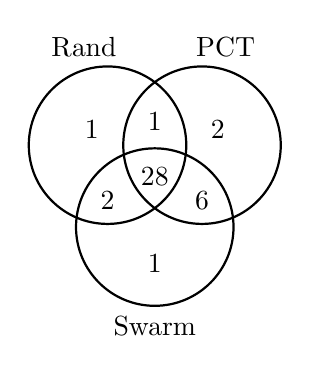
\begin{tikzpicture}[thick]
      \draw (0,0)      circle (1) node[above,shift={(-0.3,1)}] {Rand};
      \draw (1.2,0)    circle (1) node[above,shift={(0.3,1)}]  {PCT};
      \draw (.6,-1.04) circle (1) node[below,shift={(0,-1)}]   {Swarm};

      \node at (.6,-.4)  {28}; % rand  ^ pct   ^ swarm
      \node at (1.2,-.7) {6};  % pct   ^ swarm - rand
      \node at (.6,.3)   {1};  % pct   ^ rand  - swarm
      \node at (0,-.7)   {2};  % rand  ^ swarm - pct
      \node at (1.4,.2)  {2};  % pct   - rand  - swam
      \node at (-.2,.2)  {1};  % rand  - pct   - swarm
      \node at (.6,-1.5) {1};  % swarm - pct   - rand
    \end{tikzpicture}
    \caption{Basic algorithms}\label{fig:bugs-base}
  \end{subfigure}
  \begin{subfigure}{0.3\textwidth}
    \centering
    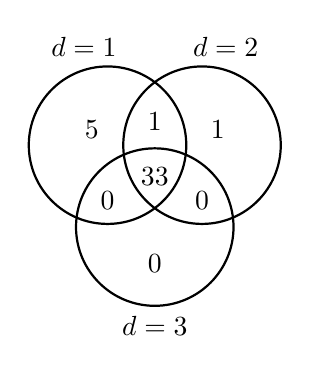
\begin{tikzpicture}[thick]
      \draw (0,0)      circle (1) node[above,shift={(-0.3,1)}] {$d=1$};
      \draw (1.2,0)    circle (1) node[above,shift={(0.3,1)}]  {$d=2$};
      \draw (.6,-1.04) circle (1) node[below,shift={(0,-1)}]   {$d=3$};

      \node at (.6,-.4)  {33}; % 1 ^ 2 ^ 3
      \node at (0,-.7)   {0};  % 1 ^ 3 - 2
      \node at (.6,.3)   {1};  % 1 ^ 2 - 3
      \node at (1.2,-.7) {0};  % 2 ^ 3 - 1
      \node at (-.2,.2)  {5};  % 1 - 2 - 3
      \node at (1.4,.2)  {1};  % 2 - 1 - 3
      \node at (.6,-1.5) {0};  % 3 - 1 - 2
    \end{tikzpicture}
    \caption{Weight changes}\label{fig:bugs-swarmd}
  \end{subfigure}

  \caption{Overlap of bugs found by each scheduling algorithm.}\label{fig:bugs}
\end{figure}

\subsection{Experimental Results}
\label{sec:algorithms-bench-results}

We conducted our experiments using an Ubuntu 12.04 virtual machine,
and a modified version of Maple based on the last commit from
2012\footnote{The same environment as \cite{thomson2016}, available at
  \url{https://github.com/mc-imperial/sctbench}}.  \Cref{lst:swarm} in
\Cref{app:swarm} shows the core of our swarm scheduling
implementation.  Other than the addition of swarm scheduling, the code
is unchanged.

The Venn diagrams in \Cref{fig:bugs} show the relative bug-finding
ability of each algorithm.  \Cref{fig:bugs-base} summarises the bugs
found by controlled random scheduling, PCT $d=3$, and swarm scheduling
$d=0$ (which we now call ``Swarm'' for brevity).  Swarm performs
comparably with PCT.  \Cref{fig:bugs-swarmd} shows the effect of
introducing weight change points, which seems to harm performance.

\begin{figure}
  \centering
  \input{gen/bugs.tex}
  \caption[Plot of bugs found by each scheduling algorithm.]{The number of bugs found by each algorithm across all benchmarks.  This plot is intended to be viewed with colour.}\label{fig:totalbugs}
\end{figure}

As the techniques we have considered are nondeterministic, it is
interesting to consider their average-case behaviour.
\Cref{fig:totalbugs} shows the aggregate behaviour of the algorithms
across all benchmarks as the number of executions increases.  Swarm
outperforms PCT at first, but PCT catches up as the number of
executions increases.

\begin{figure}
  \centering
  \begin{subfigure}{0.49\textwidth}
    \centering
    \resizebox{\textwidth}{!}{\input{gen/freqs-total.tex}}
    \caption{All buggy executions.}\label{fig:freqbugs-total}
  \end{subfigure}
  \begin{subfigure}{0.49\textwidth}
    \centering
    \resizebox{\textwidth}{!}{\input{gen/freqs-unique.tex}}
    \caption{Unique buggy executions.}\label{fig:freqbugs-unique}
  \end{subfigure}
  \caption[Plot of average number of executions needed to expose a bug.]{The average number of executions to expose a bug across all benchmarks.  These plots are intended to be viewed with colour.}\label{fig:freqbugs}
\end{figure}

The plots in \Cref{fig:freqbugs} show the average number of executions
to find a bug across all benchmarks; as expected, the average number
of executions to find \emph{any} bug rapidly converges, however the
average number of schedules to find a \emph{unique} bug does not.
This is due to two factors: (1) the number of bugs is finite; and (2)
some bugs may be out of reach of a particular algorithm.
\Cref{tbl:freqs} shows the final values.  We can see that PCT and
Swarm are almost identical, and both significantly improve upon random
scheduling when it comes to finding unique bugs.

\begin{table}
  \centering
  \begin{tabular}{lrr} \toprule
    Algorithm & Any Bug & A Unique Bug \\ \midrule
    Random & 0.071 & 312.5 \\
    PCT   & 0.077 & 270.3 \\
    Swarm & 0.078 & 270.3 \\ \bottomrule
  \end{tabular}
  \caption{Average number of executions needed to find a bug.}\label{tbl:freqs}
\end{table}

\section{Evaluation}
\label{sec:algorithms-eval}

Testing concurrent programs by using a swarm of randomly generated
weighted distributions appears to work well in practice.  The simplest
variant, which we simply call Swarm, uses no weight change points.  So
for Swarm, the $k$ and $d$ parameters are irrelevant, which means the
user does not need to know the maximum length of their program
execution in advance.  Although it is disappointing that Swarm does
not improve upon PCT, in terms of bug-finding it does perform
comparably.

A significant advantage of the Swarm method over PCT is that it does
not require the programmer to first determine the maximum length of an
execution, which can be difficult to estimate.

\paragraph{Randomised stride}
Another algorithm with a similar motivation is the randomised stride
algorithm \parencite{abdelrasoul2017}, which outperforms PCT (and so our
Swarm algorithm).  This is a recent algorithm which was not yet
published when we began this work.  Like PCT, randomised stride
derives its power from knowledge of the underlying program: in this
case, an estimate of the length of each thread.  Although Swarm
performs worse than randomised stride, we believe it still has a place
in the concurrency testing arsenal as an effective algorithm which
does not require first estimating or measuring some parameter of the
program under test.

\paragraph{Why are weight changes bad?}
\Cref{fig:bugs-swarmd} shows that, although using one weight change
point results in finding an additional bug, bug-finding ability
rapidly degrades as more points are introduced.  We suspect that this
is because frequent weight changes compromise the intuition for why
weighted random testing is effective at all.  We believe that weighted
random testing is effective because unfair scheduling causes threads
to make progress at different rates, leading to interleavings which
the programmer is unlikely to have considered.  However, by changing
weights, a thread which was previously making rapid progress may
suddenly slow down, allowing other threads to catch up.  In the
extreme, if we introduce a weight change after every scheduling point,
we have simply produced a complicated version of uniform random
scheduling.

\section{Summary}

In this chapter we presented swarm scheduling, our scheduling
algorithm for finding faults in concurrent programs:

\begin{itemize}
\item We propose that unfair schedules are likely to reveal
  concurrency bugs more effectively than fair schedules.  Unfair
  schedules cause different threads to make progress at different
  rates, resulting in interleavings the programmer is unlikely to have
  considered~\sref{algorithms-eval}.

\item Swarm scheduling uses weighted random scheduling, with optional
  weight change points.  However, frequently changing the weights
  causes weighted scheduling to degrade to an effectively uniform
  scheduling~\sref{algorithms-swarm}.

\item We find that one parameterisation of the swarm scheduling
  algorithm performs as well as PCT \parencite{burckhardt2010}, despite not
  knowing anything about the program under test.  We argue that this
  makes swarm scheduling easier to use, while giving just as good
  results~\sref{algorithms-bench}.
\end{itemize}

The complete systematic approach to testing is not necessarily
suitable for all programs.  Programs with large state-spaces, or
programs which have sources of nondeterminism other than the
scheduler, cannot readily be tested with such techniques.  For such
programs, random testing is commonly used.  By introducing swarm
scheduling, we hope that effective random testing of concurrent
programs will become simpler.

\paragraph{Context}
Swarm does not stand alone, it is related to our other contributions:

\begin{itemize}
\item \Cref{chp:dejafu} uses swarm scheduling to provide its random
  testing mode.  Complete testing is the default.  Swarm scheduling
  was added for cases where the state-space is too large to
  systematically explore.
\end{itemize}
